\subsubsection{Привести примеры различных двуполупериодных выпрямителей и сравнить их свойства}

В источниках вторичного питания необходимо использование т.н. выпрямителей сигнала. Они преобразуют переменный разнополярный сигнал в сигнал одной полярности. В неуправляемых выпрямителях широкое применение находят кремниевые полупроводниковые диоды. 

Простейший 2х п/п выпрямитель имеет вид:
\begin{center}
	\begin{figure}[h!]
		\center{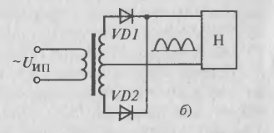
\includegraphics[scale=0.7]{s2pp.png}}
		\caption{Простейший двух п/п выпрямитель}
	\end{figure}
\end{center}

На этой схеме два диода включены встречно друг другу, $\Rightarrow$ они открыты в разные полупериоды. $U_{\textit{сети}}$ передаётся на вторую обмотку, где оно делится выводом на две составляющие $U_1$ и $U_2$.

Среднее значение напряжения на выходе получается из формулы
$$
U_{out_{med}} \approx \frac{1}{T}\left(\int \limits_0^{T/2} U_{1_m}\sin(\omega t)dt + \int \limits_0^{T/2} U_{2_m}\sin(\omega t)dt \right)
$$

Или, с допущением, что $U_1 = U_2$, 
$$
U_{out_{med}} \approx 2\frac{1}{T}\int \limits_0^{T/2} U_{m_i}\sin(\omega t)dt = 2U_{m_i}/\pi
$$
Среднее значение тока:
$$
I_{med} = \frac{U_{out_{med}}}{R_{out}}
$$

Основным недостатоком данного выпрямителя является то, что в каждый полупериод используется только часть входного напряжения. Также, следует предъявить удвоенные требования к пробивному напряжению для каждого диода по сравнению с выпрямителем на основе диодного моста, который сейчас и рассмотрим:
\begin{center}
	\begin{figure}[h!]
		\center{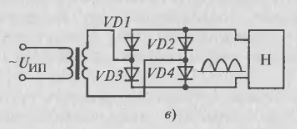
\includegraphics[scale=0.7]{DM.png}}
		\caption{двух п/п выпрямитель на основе диодного моста}
	\end{figure}
\end{center}

Вследствие лучшиъ массогабаритных и стоимостных показателей мостовой схемы ей, как правило, отдают предпочтение перед двух п/п схемой с двумя одинаковыми вторичными обмотками и выпрямительными диодами.

Нетрудно показать, что среднее значение $U_{out}$ этой схемы в два раза больше среднего значения выходного напряжения предыдущей схемы. ($\Rightarrow$ то же и для тока)

Следует заметить, что в двух п/п выпрямителях выпрямленное напряжение имеет частоту пульсаций в два раза превышающую частоту пульсации питающей цепи.

Нередко к нагрузке подключают фильтрующий конденсатор, чтобы снизить пульсации. Коэффициент пульсаций определяется в обоих случаях как
$$
K_{puls} = \frac{U_{out_{A_1}}}{U_{out_{med}}}
$$
 

